\documentclass{standalone}
\usepackage{tikz}
\begin{document}
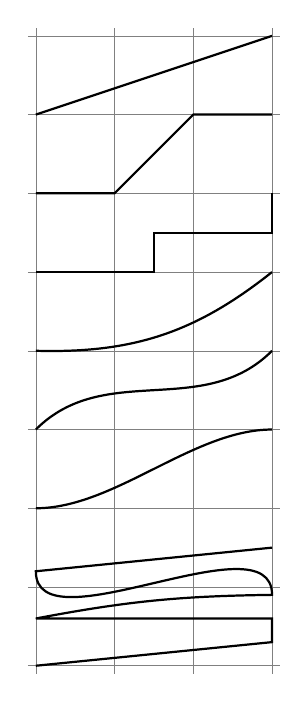
\begin{tikzpicture}[thick]
\draw[help lines] (-0.1,-0.1) grid (3.1,8.1);

% line segment
\draw (0,7) -- +(3,1);
% polyline
\draw (0,6) -- ++(1,0) -- ++(1,1) -- ++(1,0);
% orthogonal line
\draw (0,5) -| ++(1.5,0.5) -| ++(1.5,0.5);
% bent line
\draw (0,4) to[bend right=20] +(3,1);
% by in- and out-degrees
\draw (0,3) to[out=45,in=225] +(3,1);
% Bezier curve
\draw (0,2) .. controls +(1,0) and +(-1,0) .. +(3,1);

% above commands can form segments of a single path
\draw (0,0) -- ++(3,.3)
             |- ++(-3,.3)
             to[bend left=5] ++(3,.3)
             .. controls +(0,1) and +(0,-1) .. ++(-3,.3)
             -- ++(3,.3);

\end{tikzpicture}
\end{document}
